
In general, we can obtain the following lemma:
\begin{lemma}
Given the two following parallel lines:
\begin{align}
    a\vec{n}^T\vec{x} - c_1 = 0\\
    b\vec{n}^T\vec{x} - c_2 = 0
    \label{aug/2/15/ref}
\end{align}
The line equidistant from both parallel lines would be given by:
\begin{align}
    \vec{n}^T\vec{x} - \frac{1}{2}\brak{{\frac{c_1}{a} + \frac{c_2}{b}}} = 0
\end{align}
\end{lemma}
\begin{proof}
The distance between a point $\vec{A}$ and a line $L = \vec{n}^T\vec{x} - c$ is given by:
\begin{align}
    \norm{\vec{P} - \vec{A}} = \frac{\abs{\vec{n}^T \vec{A} - c}}{\norm{\vec{n}}}
\end{align}
where $\vec{P}$ is the foot of perpendicular from $\vec{A}$ onto L.\\
Consider a point $\vec{x}$ equidistant from both parallel lines, then:
\begin{align}
    \frac{\abs{a\vec{n}^T\vec{x} - c_1}}{\norm{a\vec{n}}} = 
    \frac{\abs{b\vec{n}^T\vec{x} - c_2}}{\norm{b\vec{n}}}\\
      \frac{\abs{a\vec{n}^T\vec{x} - c_1}}{\abs{a}} = 
    \frac{\abs{b\vec{n}^T\vec{x} - c_2}}{\abs{b}}\\
      \abs{ab\vec{n}^T\vec{x} - bc_1} = \abs{ab\vec{n}^T\vec{x} - ac_2}\\
      2ab\vec{n}^T\vec{x} - bc_1 - ac_2 = 0\\
      \vec{n}^T\vec{x} - \frac{1}{2}\brak{{\frac{c_1}{a} + \frac{c_2}{b}}} = 0
      \label{aug/2/15/ans}
      \end{align}
\end{proof}


The two given parallel lines can be written as:
\begin{align}
    3\myvec{3 & 2}\vec{x} - 7 = 0\\
    \myvec{3 & 2}\vec{x} + 6 = 0
\end{align}
On comparing the equations with
\eqref{aug/2/15/ref},
\begin{align}
    \vec{n} = \myvec{3 & 2}\\
    a = 3\\
    b = 1\\
    c_1 = 7\\
    c_2 = -6
\end{align}
On substituting these values into \eqref{aug/2/15/ans},
\begin{align}
    \myvec{3 & 2}\vec{x} - \frac{1}{2}\brak{\frac{7}{3} - 6} = 0\\
    \myvec{3 & 2}\vec{x} - \frac{11}{6} = 0
\end{align} 
\begin{figure}[!ht]
    See Fig. \ref{fig:aug/2/15/}.
\centering
 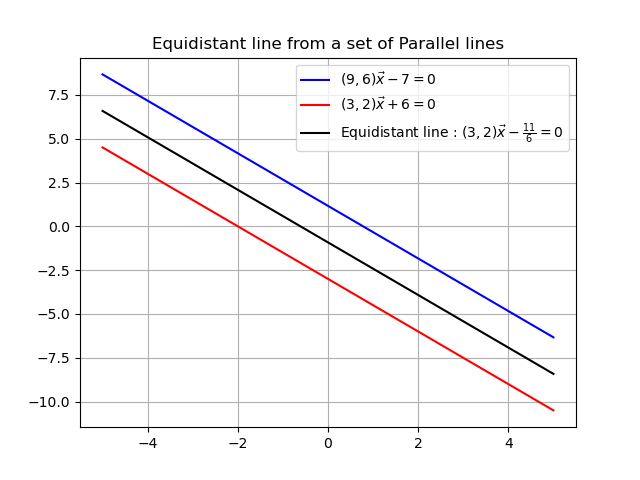
\includegraphics[width=\columnwidth]{solutions/aug/2/15/graph.png}
 \caption{The equidistant line}
 \label{fig:aug/2/15/}
 \end{figure}

